\documentclass[rnd]{mas_proposal}
% \documentclass[thesis]{mas_proposal}

\usepackage[utf8]{inputenc}
\usepackage{amsmath}
\usepackage{amsfonts}
\usepackage{amssymb}
\usepackage{graphicx}
\usepackage{array}
\usepackage[T1]{fontenc}
\usepackage{geometry}
\usepackage{booktabs}
\usepackage{tabularx}
\usepackage{enumitem}
\usepackage{titlesec}
\usepackage{hyperref}
\usepackage{svg}


\title{A Systematic Review of Human Feedback Modalities in Interactive Reinforcement Learning}
\author{Behrouz Ghamkhar}
\supervisors{Prof. Dr. Javad Ghofrani, \\
Prof. Dr. Teena Chakkalayil Hassan}
\date{September 2025}
% \thirdpartylogo{path/to/your/image}

\begin{document}

\maketitle

\pagestyle{plain}


% \thirdpartylogo{path/to/your/image}
\begin{abstract}
    A major challenge in robotics is getting robots to adapt to new, unpredictable situations. Interactive Reinforcement Learning (IRL) tries to solve this by letting humans guide the robot's learning with feedback. However, most current IRL systems use simple feedback methods like keyboard presses, which are unnatural and limit what the robot can learn. This review systematically analyzes 21 studies to map out the current methods for integrating human feedback in IRL. We found that most research focuses on basic input methods, and there is a lack of scalable, intuitive interfaces. These findings highlight a clear gap in the literature. This systematic review serves as the foundational research that directly motivates our subsequent R\&D project. The proposed project will use Virtual Reality (VR) headsets to create a natural, multi-modal feedback channel for training robots."

    \textbf{Keywords:} interactive reinforcement learning, human-robot interaction, human feedback, systematic literature review, VR interfaces, virtual reality
\end{abstract}

\section{Introduction}
Robots have the potential to become important partners in human environments, helping with tasks at home or in complex collaborative work \citep{Chetouani2021, Akalin2021}. However, it is still very difficult for robots to work well in open-world environments. These environments have unknown tasks, new objects, and dynamic human interactions. This gap highlights an important shortcoming: robots often lack the common sense and contextual understanding that humans use effortlessly to generalize their skills and interpret underspecified instructions.

A promising way to address this problem is Interactive Reinforcement Learning (IRL), which includes human feedback directly into the robot's learning loop. \citep{Lin2020, BradleyKnox2008}.This approach aims to improve sample efficiency, accelerate policy acquisition, and align the robot's behavior with human preferences and intentions \citep{Lin2020}. By learning from evaluative feedback, demonstrations, or advice, IRL agents can adapt to complex, real-world constraints more effectively than autonomous reinforcement learning agents relying only on engineered reward functions.

Despite its potential, a significant bottleneck in traditional IRL is the interface for human feedback. Most systems rely on low-bandwidth, explicit channels such as keyboard presses, button clicks, or simple GUI interactions, \citep{Faulkner2020, Loftin2014}. These methods are unnatural and awkward for the human teacher. They also cannot capture the rich details of human communication, like gestures, gaze, and tone of voice \citep{9794595, Lin2020a}. This creates an expressiveness gap, limiting the quality and type of information that can be transferred from human to robot.

At the same time, advances in consumer-grade Virtual Reality (VR) technology have created new opportunities for human-computer interaction. Modern VR headsets have many sensors that can track head pose, hand gestures, eye gaze, and voice input, offering an immersive and intuitive interface for human communication. While VR has been used for preference elicitation \cite{Heuvel2025}, its potential for capturing real-time, in-the-loop, scalar feedback within an IRL framework remains mostly unexplored. This is a missed opportunity to create a better human-robot teaching interaction.

Furthermore, a fundamental scalability challenge persists in human-in-the-loop systems. Deep RL becomes efficient by running hundreds of simulations at the same time. A human teacher cannot possibly give feedback at this scale and pace. This creates a bottleneck that stops IRL from fully using modern computing power.

To address these gaps, our subsequent R\&D project proposes a new system that uses VR headsets as a rich interface for IRL. The main idea is to let users give intuitive, immersive feedback to a virtual agent using gestures, gaze, and voice. To solve the scalability problem, we propose a two-step method: first, collecting a high-quality dataset of human feedback in VR; second, using this dataset to train a model that learns to imitate the human's feedback. This model can then generate synthetic feedback at a large scale, across many simulations. This keeps the benefits of human guidance without needing a human to be always present.

However, the field of IRL is diverse, with many different feedback modalities, algorithmic integrations, and evaluation methods documented across different communities. To the best of our knowledge, no existing systematic review has synthesized this literature with a specific focus on the characteristics of feedback integration methods and their implications for developing next-generation, immersive interfaces. Therefore, to establish a foundational understanding and clearly define the contribution of our proposed work, we first conduct a Systematic Literature Review (SLR).

The primary objective of this review is to map the current state of IRL, focusing on how human feedback is used to guide robot learning. This will help us find established methods, see the limits of current feedback systems, and strongly justify our VR-based approach. The main contributions of this review are:
\begin{enumerate}
    \item A systematic synthesis of the state-of-the-art in IRL for HRI.
    \item A clear categorization of feedback modalities, algorithms, and application domains.
    \item The identification of limitations in current feedback methods, highlighting the expressiveness and scalability gaps.
    \item The formulation of research questions to guide future work, including our proposed VR-based approach.
\end{enumerate}

To guide our work, we formulate the following research questions, using the SPIDER and PICO frameworks:

\begin{itemize}
    \item \textbf{SPIDER:} What are the predominant algorithms, reward function designs, and human feedback integration modalities used in IRL for HRI, and how are they characterized and evaluated?
    \item \textbf{PICO:} In IRL systems for human-robot interaction (Population), what are the effects of implementing specific algorithms, reward designs, and feedback modalities (Intervention) compared to alternative approaches (Comparison) on system performance, learning efficiency, and task outcomes (Outcome)?
    
\end{itemize}

The rest of this paper is structured as follows: Section \ref{sec:related} (Related Work) presents relevant literature, existing survey papers, and identifies limitations in current research that motivate this study. Section \ref{sec:methodology} (Methodology) details our systematic approach, including search strategy, selection criteria, and data extraction process using our structured survey tool. Section \ref{sec:analysis} (Analysis) provides both descriptive statistics and thematic synthesis of the findings, addressing our research questions through comparative evaluation of the included studies. Section \ref{sec:discussion} (Discussion) interprets the results, examines limitations and potential biases, and explores contradictory findings within the literature. Section \ref{sec:future} (Future Research Directions) identifies emerging trends, research gaps, and under-investigated areas in the field. Finally, Section \ref{sec:conclusion} (Conclusion) summarizes key findings, reflects on the research questions, and provides final remarks on the state of IRL in HRI.

\section{Related Work}
\label{sec:related}

\subsection{Relevant Literature}
The foundation of this review is based on important papers that shaped the IRL field. Key work by \citet{BradleyKnox2008} introduced TAMER, showing that human evaluative feedback could train agents much faster than autonomous RL. This was extended into social domains by \citet{Lin2020a} and \citet{Lin2020}, who reviewed and implemented systems using implicit social feedback like facial expressions and gestures. Research into handling imperfect teachers was advanced by \citet{Faulkner2020} and \citet{KesslerFaulkner2021}, while the fusion of multi-modal advice was explored by \citet{9794595}. The potential of physiological signals was shown by \citet{Xu2021}, who used EEG-based feedback. Most recently, \citet{Heuvel2025} began exploring immersive interfaces, comparing VR and 2D for preference-based learning. This study is very close to our proposed research.

\subsection{Existing Survey Papers and Secondary Studies}
This SLR builds on and expands upon existing secondary studies. The comprehensive review by \citet{Lin2020} provides an excellent overview of learning from human social feedback, categorizing algorithms like TAMER and COACH. \citet{Chetouani2021} offers a broader overview of interactive robot learning, covering feedback, demonstrations, and instructions. \citet{Akalin2021} surveys RL applications specifically in social robotics, focusing on reward design and evaluation. This current review differentiates itself by including the latest studies up to 2025, providing a detailed technical analysis of algorithms and reward structures from the collected papers, and explicitly framing the analysis to identify the gap for rich, VR-based feedback interfaces.

\subsection{Overview of Topics in Related Work}
The literature shows several core topics in IRL:
\begin{enumerate}
    \item \textbf{Algorithmic Approaches}: including value-based methods (Q-learning, DQN), policy-based methods (Policy Shaping), and actor-critic methods (SAC), often adapted to incorporate human input.
    \item \textbf{Feedback Modalities}: ranging from explicit (keyboard, GUI, verbal commands) to implicit (EEG, gaze, gestures) feedback.
    \item \textbf{Reward Design}: a critical challenge, with solutions including human feedback as reward shaping, inverse RL from demonstrations, and complex composite functions. 
    \item \textbf{Application Domains}: including social robotics (e.g., \citet{Akalin2021}), industrial collaboration, rehabilitation, and virtual agent training.
\end{enumerate}

\begin{figure}[h!]
\centering
\includesvg[width=\linewidth]{images/mindmap_svg.svg}
\caption{A mindmap showing the categorization of the 21 reviewed studies on IRL in HRI. The map is structured along five primary dimensions: Feedback Modality, Algorithmic Approach, Application Domain, Evaluation Method, and Research Focus. The MindMup web application (www.mindmup.com) was used to create this mind map.}
\label{fig:alg_dist}
\end{figure}

\subsection{Limitations of Existing Work and Motivation for Current Research}
Despite these advances, key problems remain, forming the motivation for our subsequent R\&D project. First, an expressiveness gap exists; most systems rely on low-bandwidth inputs like keyboard buttons (\citet{Faulkner2020, Loftin2014}), which are unnatural and fail to capture the details of human communication. Second, a scalability bottleneck is inherent to human-in-the-loop systems; they cannot parallelize across hundreds of environments like modern Deep RL. Third, the use of VR interfaces is very new; while used for demonstrations and preferences (\citet{Heuvel2025}), its potential for real-time, in-loop \textit{scalar} feedback remains almost entirely unexplored. Finally, the fusion of multi-modal signals from VR (gaze, pose, gesture) into a robust reward signal is an unresolved challenge. Our research aims to address these specific deficits.

\section{Methodology}
\label{sec:methodology}
We carried out this systematic literature review using standard academic guidelines. This ensured a structured, clear, and repeatable process. We followed the well-known PRISMA (Preferred Reporting Items for Systematic Reviews and Meta-Analyses) framework to report the review.

\subsection{Search Procedure}
We used two methods to find relevant academic papers: a systematic keyword search across major digital libraries and an extra snowballing search. Using both methods is recommended to get complete coverage of the literature.

The first step was an electronic search using a specific Boolean query. The search terms were chosen to find studies about Interactive Reinforcement Learning, human feedback, and Human-Robot Interaction
\begin{paragraph}
("interactive reinforcement learning" OR "human-in-the-loop rl" OR "irl" OR "interactive RL") 
AND 
("human feedback" OR "human evaluation" OR "human reward" OR "human guidance") 
AND 
("human-robot interaction" OR "hri" OR "social robot*")  
\end{paragraph} \\

We searched four major academic databases: IEEE Xplore, ACM Digital Library, ResearchGate, and Google Scholar. We chose these platforms because they cover the relevant fields of computer science, robotics, and artificial intelligence well.

To make sure we didn't miss any key papers, we also did a snowballing search. This meant looking at the reference lists of important papers from the first search, especially previous review articles and highly cited works.

The full process of identification, including the final number of records from each source, is shown in the PRISMA flow diagram in Section~\ref{sec:prisma}.

\subsection{Inclusion/Exclusion Criteria}
We filtered the studies using the following criteria:

Before starting the selection process, we set clear rules to decide which studies to include or exclude. We defined these criteria early to reduce bias and make sure the study selection could be repeated.

The inclusion criteria required that publications must be:
\begin{itemize}
    \item Peer-reviewed conference papers, journal articles, or book chapters.
    \item Published in the English language.
    \item Published between the years 2008 and 2025.
    \item Primarily focused on applying Interactive Reinforcement Learning in a Human-Robot Interaction context.
    \item Involve some form of active human feedback to guide the robot's learning process.
\end{itemize}
Conversely, we excluded publications if they were:
\begin{itemize}
    \item Grey literature (unless explicitly included).
    \item Studies not peer-reviewed (e.g., blogs, editorials, opinion pieces).
    \item Studies unrelated to interactive contexts.
    \item Duplicates or secondary publications of the same work.

\end{itemize}

These criteria were applied in a two-stage screening process. The results of this screening are shown in the PRISMA flow diagram in Section~\ref{sec:prisma}.

\subsection{Structure of Survey Tool}
We extracted data using a structured Excel sheet. Each row in the spreadsheet was for one primary study, and the columns captured the key aspects of the research as defined in the first row of the provided file. The main categories include:
\begin{itemize}
    \item Bibliographic information: ID, Title, Author, Year, DOI/URL, Publication Venue
    \item Research characteristics: Research Question, RL Algorithm Type, Reward Function Design, Training Method
    \item HRI-specific elements: Human Feedback Integration, Interaction Modality, Transparency/Explainability, Adaptation to Human Behavior, HRI Scenario, Learning Objective
    \item Experimental setup: Robot Type, Environment (real/simulated), Simulation Tools, Physical Experiment Setup
    \item Evaluation approach: Evaluation Method, Evaluation Metrics, Participants
    \item Study outcomes: Limitations, Results
\end{itemize}

The complete survey tool with all extracted data is available as part of our supplementary materials.

\subsection{PRISMA Flow Diagram}
\label{sec:prisma}
The study selection process is summarized in the PRISMA flow diagram Figure ~\ref{fig:prisma}, which shows the number of records identified, screened, assessed for eligibility, and finally included in the systematic review.

\begin{figure}[h!]
\centering
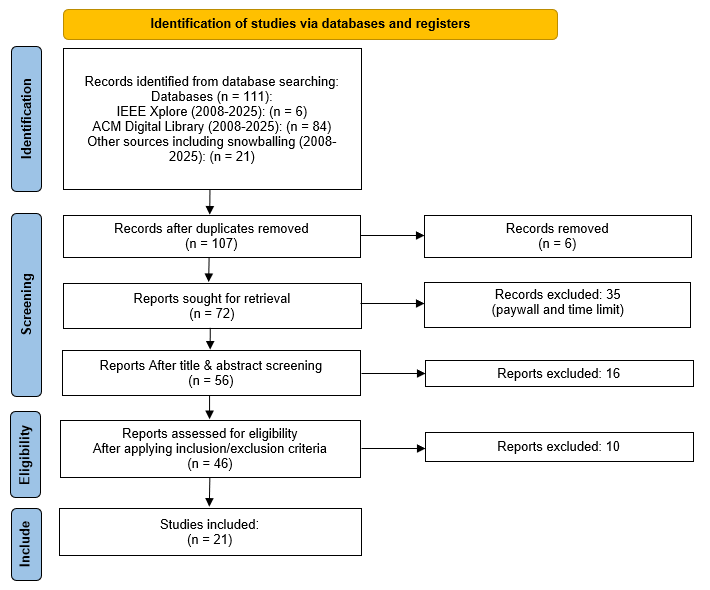
\includegraphics[width=0.8\textwidth]{images/prisma.PNG}
\caption{PRISMA Flow Diagram of the study selection process.}
\label{fig:prisma}
\end{figure}

\textbf{Identification Phase:} Our first search across the selected databases (IEEE Xplore and ACM Digital Library) found 90 records. We found another 21 records through other sources, including snowballing (looking at references and citations of selected studies). This gave a total of 111 records for screening.

\textbf{Screening Phase:} After removing 6 duplicate records, 107 unique records remained. Of these, we could not get the full text of 35 records due to practical problems, mainly paywalls and time limits. We screened the titles and abstracts of the remaining 72 records against our inclusion and exclusion criteria. This led to the exclusion of 16 records that were not about IRL or HRI.

\newcolumntype{L}[1]{>{\raggedright\let\newline\\\arraybackslash\hspace{0pt}}p{#1}}
\begin{table}
\centering
\scriptsize
\begin{tabular}{|L{0.3cm}|L{5.5cm}|L{2cm}|L{0.6cm}|L{1.8cm}|L{2.2cm}|}
\hline
\textbf{ID} & \textbf{Title} & \textbf{Author} & \textbf{Year} & \textbf{Journal/Conference} & \textbf{RL Algorithm} \\
\hline
\cite{Akalin2021} & Reinforcement Learning Approaches in Social Robotics & Akalin, Loutfi & 2021 & Sensors & Various (Q-learning, DQN, etc.) \\
\hline
\cite{Alzahrani2025} & Optimising Human Trust in Robots: A Reinforcement Learning Approach & Alzahrani, Ahmad & 2025 & ACM/IEEE HRI & Q-learning \\
\hline
\cite{BradleyKnox2008} & TAMER: Training an Agent Manually via Evaluative Reinforcement & Knox, Stone & 2008 & IEEE ICDL & Supervised Learning \\
\hline
\cite{Chetouani2021} & Interactive Robot Learning: An Overview & Chetouani & 2021 & Lecture Notes in Computer Science & Interactive RL, Inverse RL \\
\hline
\cite{Heuvel2025} & The Impact of VR and 2D Interfaces on Human Feedback in Preference-Based Robot Learning & de Heuvel et al. & 2025 & IEEE/RSJ IROS & TD3 (actor-critic) \\
\hline
\cite{Escontrela2022} & Adversarial Motion Priors Make Good Substitutes for Complex Reward Functions & Escontrela et al. & 2022 & IEEE/RSJ IROS & AMP + RL \\
\hline
\cite{Faulkner2020} & Interactive reinforcement learning with inaccurate feedback & Faulkner et al. & 2020 & IEEE ICRA & Policy Shaping, TAMER+RL \\
\hline
\cite{GonzalezSantocildes2024} & Adaptive Robot Behavior Based on Human Comfort Using Reinforcement Learning & Gonzalez-Santocildes et al. & 2024 & IEEE Access & SAC (Soft Actor Critic) \\
\hline
\cite{KesslerFaulkner2021} & Interactive Reinforcement Learning from Imperfect Teachers & Kessler Faulkner, Thomaz & 2021 & ACM/IEEE HRI & Policy Shaping variants \\
\hline
\cite{Lin2020} & A Review on Interactive Reinforcement Learning From Human Social Feedback & Lin et al. & 2020 & IEEE Access & TAMER, COACH, Deep TAMER \\
\hline
\cite{Lin2020a} & Human Social Feedback for Efficient Interactive Reinforcement Agent Learning & Lin et al. & 2020 & IEEE RO-MAN & TAMER \\
\hline
\cite{Loftin2014} & Learning something from nothing: Leveraging implicit human feedback strategies & Loftin et al. & 2014 & IEEE RO-MAN & Strategy-Aware Bayesian Learning \\
\hline
\cite{Luo2024} & Real-Time Simulated Avatar from Head-Mounted Sensors & Luo et al. & 2024 & IEEE/CVF CVPR & PPO (teacher policy) \\
\hline
\cite{Moreira2020} & Deep reinforcement learning with interactive feedback in a human--robot environment & Moreira et al. & 2020 & Applied Sciences & Deep Q-Learning (DQN) \\
\hline
\cite{MunguiaGaleano2023} & Affordance-Based Human–Robot Interaction With Reinforcement Learning & Munguia-Galeano et al. & 2023 & IEEE Access & Contextual Q-learning \\
\hline
\cite{8624972} & User Feedback in Latent Space Robotic Skill Learning & Pahič et al. & 2018 & IEEE Humanoids & Policy search (PoWER) \\
\hline
\cite{6147010} & Augmented Reinforcement Learning for Interaction with Non-expert Humans in Agent Domains & Sridharan & 2011 & IEEE ICMLA & Policy Gradient, Cross-Entropy \\
\hline
\cite{9794595} & Interactive Reinforcement Learning With Bayesian Fusion of Multimodal Advice & Trick et al. & 2022 & IEEE Robotics and Automation Letters & Tabular Q-Learning \\
\hline
\cite{Winkler2022} & QuestSim: Human Motion Tracking from Sparse Sensors with Simulated Avatars & Winkler et al. & 2022 & SIGGRAPH Asia & PPO \\
\hline
\cite{Xu2021} & Accelerating Reinforcement Learning using EEG-based implicit human feedback & Xu et al. & 2021 & Neurocomputing & Bayesian Deep Q-Network \\
\hline
\cite{Ye2022} & Neural3Points: Learning to Generate Physically Realistic Full-body Motion for Virtual Reality Users & Ye et al. & 2023 & Computer Graphics Forum & PPO \\
\hline
\end{tabular}
\caption{Part of the Survey Tool Structure (The full table with all 21 papers and all columns is in the attached Excel file)}
\label{tab:survey_tool}
\end{table}

\textbf{Eligibility and Inclusion Phase:} We tried to get the full text of 56 reports. We assessed these for eligibility by reading the full text. After applying the inclusion and exclusion criteria, we excluded 10 reports that did not meet the study's requirements. This process led to the selection of 21 papers out of the remaining 46 for inclusion in the final SLR.

\section{Analysis}
\label{sec:analysis}

\subsection{Descriptive Analysis}
The 21 papers were published between 2008 and 2025. More papers were published in recent years, showing growing interest in the field. The most common places to publish were IEEE Access, the HRI conference, and ICRA.
A deep look at the algorithms shows a field that adapts basic Reinforcement Learning (RL) methods to the special challenges of human-in-the-loop training. The choices are not random but are strategic, based on the type of human feedback and the learning task.


\subsubsection{Value-Based Methods: Stability and Integration}
Value-based methods, especially Q-learning and its variants, are the most common type, found in 8 out of 21 studies. They are popular because they are well-understood, stable in discrete action spaces, and it is straightforward to add human feedback to them.
\begin{itemize}
    \item Standard \& Contextual Q-Learning: The foundational tabular Q-learning algorithm is effectively employed in simpler, discrete state-action tasks, such as the sequential object selection task in \citet{9794595} and the grid-world navigation and trust optimization in \citet{Alzahrani2025}. Its simplicity makes the impact of human advice or reward shaping directly observable. \citet{MunguiaGaleano2023} uses a Contextual Q-learning (CQL) approach to leverage affordances, demonstrating how classic value-based methods can be extended for more complex, context-aware HRI.
    \item Deep Q-Networks (DQN): For higher-dimensional state spaces (e.g., pixel inputs in simulated environments), Deep Q-Networks are the natural evolution. \citet{Moreira2020} uses a DQN with a CNN for an object-sorting task, while \citet{Xu2021} develops a more advanced Bayesian Deep Q-Network (BDQN) to robustly integrate the uncertainty inherent in EEG-based implicit feedback. This shows a trend where value-based methods are scaled using deep learning while maintaining their core principle of learning an action-value function.
\end{itemize}


\subsubsection{Policy Search and Policy Gradient Methods: Direct Optimization}
Policy Search methods, found in 5 studies, directly optimize the policy parameters. This approach is often chosen for continuous control tasks common in robotics, like manipulation and locomotion.
\begin{itemize}
    \item Policy Learning by Weighting Exploration with Returns (PoWER): This algorithm is a key part of policy search in robotics. \citet{8624972} uses PoWER in a latent space to learn a ball-throwing skill, demonstrating how policy search can be effectively guided by discrete human ratings instead of engineered rewards.
    \item Policy Gradient and Cross-Entropy Method: These are foundational policy optimization techniques. \citet{6147010} uses Policy Gradient and Cross-Entropy methods in their "Augmented RL" framework, showcasing their utility for online weight adaptation between human and environmental rewards. This highlights a key strength: the direct coupling between human feedback (which often critiques the policy) and the policy update rule.
\end{itemize}

\begin{figure}[h!]
\centering
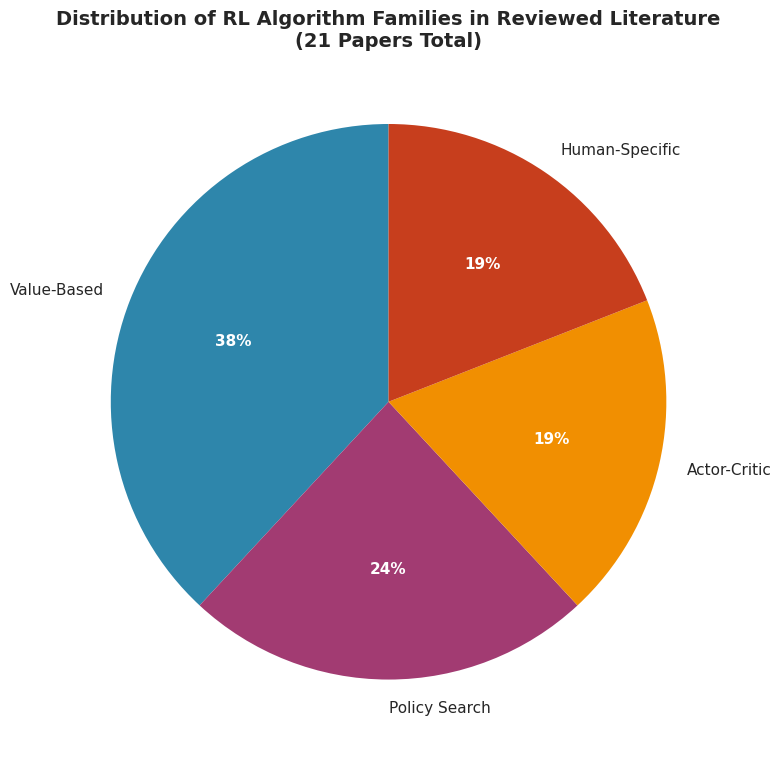
\includegraphics[width=0.7\linewidth]{images/algorithm_distribution_pie.png}
\caption{Proportional distribution of primary algorithm families identified in the systematic review. Value-based methods constitute the largest category (38\%), underscoring their established role in interactive reinforcement learning for human-robot interaction. The combined prevalence of policy search and human-specific frameworks (43\%) highlights the field's significant focus on algorithms designed for direct policy optimization and specialized human feedback integration.}
\label{fig:algorithm_distribution}
\end{figure}

\subsubsection{Actor-Critic and Advanced Methods} Complexity and Continuous Control
Actor-Critic methods, which combine value function and policy learning, are used in 4 studies tackling complex, continuous control problems. Their ability to handle high-dimensional action spaces makes them suitable for modern robotic simulation.
\begin{itemize}
    \item Proximal Policy Optimization (PPO): A modern actor-critic algorithm known for its stability, PPO is used in several advanced physics-based simulation studies. It is used for human motion tracking and avatar control in \citet{Winkler2022}, \citet{Ye2022}, and \citet{Luo2024}. In these works, PPO is not typically interactive with a human during training but is used in an imitation learning setting, often trained on motion capture (MoCap) data, which can be seen as a form of offline human demonstration.
    \item Soft Actor-Critic (SAC): An algorithm that maximizes both expected return and entropy (promoting exploration), SAC is used by \citet{GonzalezSantocildes2024} for its sample efficiency and robustness in learning comfort-aware robot behaviors. Its off-policy nature makes it well-suited for learning from the potentially expensive data gathered in HRI experiments.
\end{itemize}



\begin{figure}[h!]
\centering
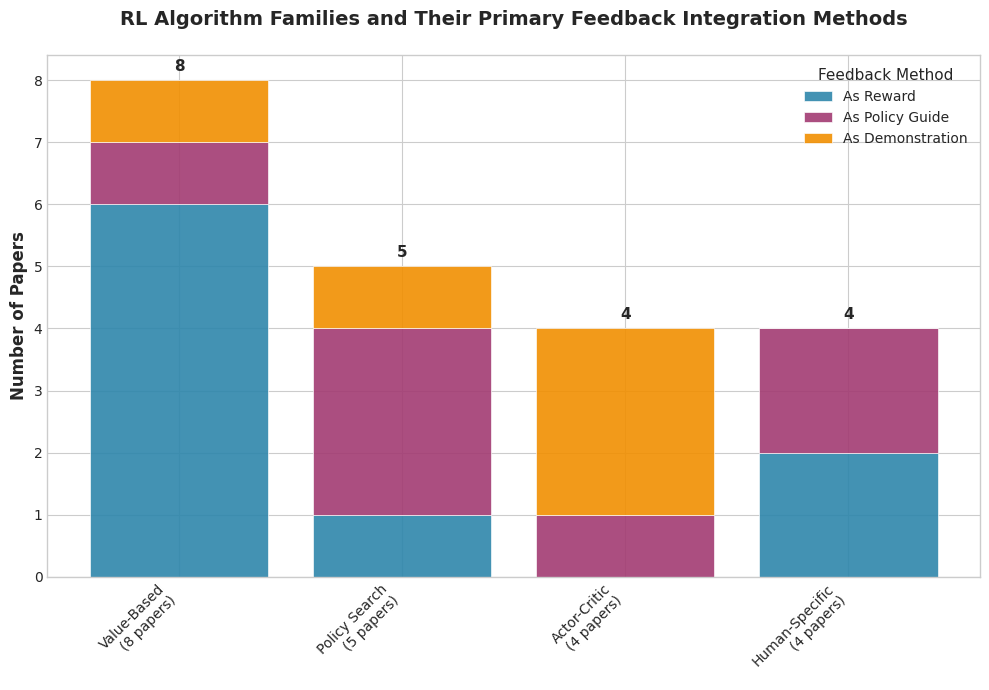
\includegraphics[width=0.85\linewidth]{images/algorithm_analysis_stacked.png}
\caption{Distribution of reinforcement learning algorithm families and their primary method for integrating human feedback across the reviewed literature ($n=21$). The analysis reveals a prevalence of value-based methods, most commonly used for reward shaping. In contrast, actor-critic methods are predominantly applied in learning from demonstration scenarios, reflecting their suitability for complex, continuous control tasks.}
\label{fig:algorithm_families}
\end{figure}


\subsubsection{Human-Feedback-Specific Frameworks}
A large part of the literature does not use a standard RL algorithm as its core. Instead, it builds a dedicated framework around human input.

\begin{itemize}
    \item TAMER (Training an Agent Manually via Evaluative Reinforcement): Introduced by \citet{BradleyKnox2008}, TAMER is a key framework that uses supervised learning to model a human's reward function from scalar feedback. It is not RL in the traditional sense but is a cornerstone of IRL. Its influence is clear in studies like \citet{Lin2020a}, which adapts its principles to interpret social feedback, and \citet{Faulkner2020}, which combines it with RL.
    \item Policy Shaping \& Algorithm-Agnostic Frameworks: Several studies, such as \citet{Faulkner2020} and \citet{KesslerFaulkner2021}, propose meta-frameworks like REPaIR and AMPS. These are designed to filter or interpret human feedback and can be layered on top of various underlying RL algorithms (often Q-learning or policy gradients), making them flexible tools for handling imperfect teachers.
\end{itemize}

\noindent
In summary, the analysis of the extracted data shows several key trends:
\begin{itemize}
    \item \textbf{RL Algorithms:} Q-learning and its variants (including Deep Q-Networks) are the most common (8/21 studies), followed by Policy Search methods (5/21) and Actor-Critic methods like PPO and SAC (4/21). This shows a preference for well-understood, stable algorithms that can be more easily integrated with human input.
    \item \textbf{Feedback Modality:} Explicit feedback (e.g., keyboard, GUI, button presses) is the most prevalent (12/21 studies). However, a significant portion (7/21) explores implicit or social feedback, such as gestures, facial expressions (\citet{Lin2020a}), and EEG signals (\citet{Xu2021}), highlighting a trend towards more natural interaction.
    \item \textbf{HRI Scenarios:} The applications are diverse. "Socially assistive" and "task learning" scenarios are the most common (6/21 each), followed by "collaborative manipulation" (4/21) and "locomotion/navigation" (3/21). This shows IRL's applicability across both social and functional domains.
\end{itemize}

\begin{figure}[h!]
\centering
% \includegraphics[width=0.6\textwidth]{algorithm_distribution.png} % Placeholder for a chart
\caption{Descriptive Analysis: Distribution of Primary RL Algorithms Used in the Reviewed Studies.}
\label{fig:alg_dist}
\end{figure}


\subsection{Synthesis of Knowledge}
\subsubsection{Thematic Analysis of the Research Question}
The analysis is structured around the predefined Research Question (RQ).

\textbf{RQ:} What are the predominant algorithms, reward function designs,
and human feedback integration modalities used in IRL for HRI, and how
are they characterized and evaluated?

The synthesis is organized into the following thematic areas that collectively address this question:

\begin{itemize}
\item \textbf{Algorithms and Reward Design}\\
The review finds that algorithm choice is heavily influenced by the feedback type. For explicit, evaluative feedback (e.g., +1/-1), methods like TAMER (a supervised learner) and Policy Shaping are dominant. For integrating feedback into the value function, Q-learning variants are common. Reward functions are highly diverse. A major theme is \textit{reward shaping}, where human feedback is directly used as a reward signal or combined with environmental rewards (e.g., \citet{Xu2021}). Other designs are \textit{composite functions} balancing task performance and human metrics (e.g., comfort in \citet{GonzalezSantocildes2024}, trust in \citet{Alzahrani2025}).
\item \textbf{Feedback Integration and Modalities}\\
Human feedback is integrated in three primary ways: 
\begin{enumerate}
    \item \textbf{As a reward signal} (e.g., TAMER, \citet{BradleyKnox2008}). 
    \item \textbf{As a policy guide} (e.g., Policy Shaping, \citet{Faulkner2020}). 
    \item \textbf{As a demonstration} for Inverse RL or imitation learning.
\end{enumerate}
The modalities range from low-bandwidth (keyboard) to high-bandwidth (multi-modal fusion of speech and gestures in \citet{9794595}). A clear trend is the exploration of more passive, implicit methods (EEG, gestures) to reduce the burden on the human teacher.
\item \textbf{HRI Scenarios and Evaluation}\\
Evaluation has two parts: 
\begin{enumerate}
    \item \textbf{Algorithmic performance} measured by cumulative reward, success rate, convergence speed.
    \item \textbf{HRI performance} measured by task completion time, human satisfaction, and specific metrics like comfort or trust level.
\end{enumerate}
An important finding is that many studies use simulation (15/21 papers did evaluations mostly or entirely in simulation), indicating a gap in real-world validation of these systems.
\item \textbf{Limitations and Future Directions}\\
The most common limitations mentioned in the papers are:
\begin{itemize}
    \item Small sample sizes in human studies.
    \item Simplicity of tasks and state/action spaces.
    \item The challenge of noisy, inaccurate, or delayed human feedback.
    \item The lack of long-term interaction studies.
\end{itemize}
The most common suggestion for future work is to explore more natural and intuitive feedback interfaces. This directly supports our work on VR.

\end{itemize}

\subsubsection{Comparative Analysis Across Studies}
Comparing the seminal TAMER work \citet{BradleyKnox2008} with recent studies like \citet{Heuvel2025} shows a clear evolution: from simple, discrete tasks and feedback to complex, continuous domains and rich, multi-modal interfaces. Studies using implicit feedback (\citet{Xu2021}) consistently report that it is less mentally demanding for humans but have problems with signal reliability. Meanwhile, studies focusing on algorithm robustness (\citet{Faulkner2020, KesslerFaulkner2021}) show better performance with imperfect teachers but often at the cost of increased complexity.

\section{Discussion}
\label{sec:discussion}

The field of IRL for HRI has grown from showing that human feedback can speed up learning to now tackling advanced challenges like multi-modal fusion, dealing with teacher inattentiveness, and optimizing human states like trust and comfort.

Our analysis shows a strategic matching of algorithms with feedback types. For instance, TAMER and Policy Shaping are most common for direct evaluative feedback \citep{BradleyKnox2008, Faulkner2020}, while Q-learning variants are commonly used to integrate feedback into the value function, and composite reward functions are designed to balance task performance with human metrics like comfort \citep{GonzalezSantocildes2024} and trust \citep{Alzahrani2025}.

Several limitations and problems are clear. The strong focus on simulation, while good for development, raises questions about how well these algorithms would work in the real world. Also, the variety of tasks, algorithms, and evaluation metrics makes it hard to compare studies directly, which limits meta-analysis. A key finding is the paradox of aiming for natural interaction while still mostly using unnatural feedback methods like keyboards and GUIs \citep{Faulkner2020, Loftin2014, Moreira2020}. This shows a significant disconnect between the goal of HRI and the current methods, which supports the need for our proposed R\&D project. Although promising, work on more implicit feedback like EEG \citep{Xu2021} or social cues \citep{Lin2020a} currently has problems with reliability and often does not work as well as simpler, explicit methods.

We must consider potential biases. Publication bias is a possibility; studies with positive results (showing that human feedback improves performance) are more likely to be published than those with negative or unclear results. Our search strategy, while thorough, may have missed relevant studies not in English or in less known publications. Time limits meant we searched only a few databases; searching more specialized databases might have found more papers. The analysis was also limited by the information in the published papers; some details about how things were done or negative results may have been left out.

We did not find major contradictions, but a clear result is the progression from simple, discrete tasks to exploring rich, multi-modal interfaces, as seen in the recent work by \citet{Heuvel2025} that tests VR for preference feedback. This work, along with studies focused on making algorithms robust to imperfect teachers \citep{Faulkner2020, KesslerFaulkner2021}, shows the field is moving towards more natural and scalable human-robot teaching. However, the ongoing scalability bottleneck and the expressiveness gap confirm that the goal of truly natural HRI with IRL is still a challenge. This is a challenge that our next work on VR-based feedback aims to address directly.



\subsection{Future Research Directions}
\label{sec:future}

Based on the analysis of limitations and trends, we suggest the following future research directions:
\begin{enumerate}
    \item \textbf{Natural and Immersive Feedback Interfaces:} There is a critical need to move beyond keyboards and GUIs. Research should focus on using VR/AR, advanced computer vision (for gesture and affect recognition), and physiological sensing (EEG, EMG) to create intuitive, high-bandwidth feedback channels. Our proposed project on VR-based feedback is a direct contribution to this direction.
    \item \textbf{Scalability and Parallelization:} A major gap is the inability to scale human-in-the-loop training. Future work must investigate methods like \textit{predictive human feedback models} (learning a model of the human's feedback policy) to generate synthetic feedback, enabling large-scale parallel training while retaining human-aligned behavior.
    \item \textbf{Long-term and Real-World Validation:} Research must transition from short-term, simulated studies to long-term deployments in real-world settings (homes, hospitals, factories). This will require addressing challenges like non-stationary human behavior, safety, and reward function drift over time.
\end{enumerate}

Specific areas and research gaps include exploring \textit{multi-human feedback} (how to combine feedback from multiple teachers) and \textit{explainable IRL} (helping the human understand why the agent is making certain requests for feedback).

Areas that need more investigation include using IRL for \textit{pro-social behavior} (e.g., fairness, empathy) and its use in very sensitive areas like \textit{child-robot interaction} or \textit{cognitive rehabilitation}.

\section{Conclusion}
\label{sec:conclusion}

This systematic review reveals a central paradox in IRL for HRI: the field aims to create natural human-robot teaching interactions yet remains predominantly reliant on unnatural, low-bandwidth feedback interfaces like keyboards and GUI buttons. This expressiveness gap, identified as a major limitation across the literature, presents a significant barrier to the wider adoption of IRL in real-world applications. Our work was guided by two research questions formulated using the SPIDER and PICO frameworks, focusing on characterizing the state of the art and evaluating the effects of different IRL interventions. To answer these questions, we employed a PRISMA-guided methodology (Section~\ref{sec:methodology}), systematically identifying, screening, and analyzing relevant literature.

Our analysis was based on a collection of 21 primary studies published between 2008 and 2025. The key findings from our analysis are:
\begin{itemize}
\item \textbf{Algorithmic Trends:} There is no single dominant algorithm, but a clear trend of pairing algorithm classes with feedback types. Q-learning and its variants are prevalent for value-based integration, Policy Shaping and TAMER for direct policy guidance, and actor-critic methods like PPO and SAC for complex, continuous control tasks.
\item \textbf{Reward Design Sophistication:} A significant evolution is observed in reward functions, moving from simple task-completion rewards to complex composite functions that explicitly optimize human subjective states, such as comfort \citep{GonzalezSantocildes2024} and trust \citep{Alzahrani2025}.
\item \textbf{The Feedback Paradox:} The most important finding is the strong, contrast between the goal of natural interaction and the predominant use of low-bandwidth, explicit feedback interfaces like keyboards and GUIs. This creates a significant expressiveness gap (Section~\ref{sec:discussion}).
\item \textbf{The Simulation Bottleneck:} A heavy reliance on simulated environments for evaluation questions the real-world robustness and generalizability of many proposed IRL algorithms. This shows a clear gap between simulation and reality.
\end{itemize}

As discussed in Section~\ref{sec:future}, the analysis of these findings directly points to several important future research directions. The most important is the development of natural and immersive feedback interfaces, such as VR and AR, to close the expressiveness gap, a direction recently and promisingly explored by \citet{Heuvel2025}. Secondly, to overcome the human bottleneck in large-scale Deep RL training, research must investigate scalability solutions like predictive human feedback models. Finally, the field must focus on long-term, real-world testing to move these technologies from labs to practical applications.

This review itself is not without limitations, as noted in Section~\ref{sec:discussion}. The potential for publication bias, the focus on English-language publications, and the differences between studies that make direct comparison difficult are all factors that shape our results. However, this review successfully achieves its goals: it gives a complete picture of the IRL field, clearly categorizes the state of the art, and finds the most pressing research gaps.

In conclusion, while IRL is a powerful method for creating sample-efficient and human-aligned agents, the field is still limited by simple interfaces and a scalability problem. The findings of this review provide a solid base and a clear reason for our next work on "Interactive Reinforcement Learning with Human Feedback Collected through VR Headsets." This work aims to solve these identified challenges directly.

\nocite{*}

\bibliographystyle{plainnat} % Use the plainnat bibliography style
\bibliography{bibliography.bib} % Use the bibliography.bib file as the source of references

\end{document}